\section{Part I}\label{P1}

\subsection{8-point algorithm function (version 1)}

In order to implement this algorithm, it is essential to initially construct the "A" matrix for the linear homogeneous system. To accomplish this, the \texttt{EightPointsAlgorithm(P1, P2)} function is invoked with the corresponding points $P1$ and $P2$. Subsequently, the Singular Value Decomposition ($\text{SVD}(A) = [U \ D \ V]$) is employed to produce the unit matrix $V$ and to identify the final column of $V$ as the solution, which is a $9 \times 1$ vector. For the $F$ matrix to be constructed, the subsequent step is to restructure the $9 \times 1$ matrix into a $3 \times 3$ matrix using \texttt{reshape( , [3 3])}. The matrix $F$ must have rank 2, and we manually achieve this. Using the $\text{SVD}(F) = [U \ D \ V]$, we then set $D[3,3]$ of the matrix $D$ to 0. The $F$ matrix is subsequently recomputed using $U D V^T$, in which $D[3,3]$ is equal to zero.

\subsection{8-point algorithm function (version2)}

The normalized eight-point algorithm is employed to improve the accuracy of the fundamental matrix estimation. Initially, the input points are normalized, and the eight-point algorithm from the final section is implemented. The previous algorithm's stages will be executed once more on the normalized corresponding points in the \texttt{EightPointsAlgorithmN(P1, P2)}. In order to emphasize the point, $P1$ and $P2$ must be normalized using the \texttt{normalise2dpts(P1)} function. Subsequently, the new $F$ is generated by denormalizing the functionality matrix $F$ using the \texttt{EightPointsAlgorithm(P1, P2)}. 

It is imperative to emphasize that all of the points are presented in a uniform manner. The numerical stability of the solution can be enhanced by normalizing the input points, which is involved in the solution of a linear system of equations in the 8-point algorithm. It aids in the prevention of problems associated with ill-conditioned matrices that may occur when dealing with large or small numbers in the input data. The algorithm becomes less susceptible to anomalies and noise in the data by establishing a common scale for the point coordinates. The fundamental matrix is defined to scale. The algorithm's scale-invariance is guaranteed by normalizing the coordinates. Normalization facilitates the optimization process by facilitating the attainment of more dependable and expedited convergence. It can enhance the solution's robustness, particularly in situations where the point correspondences exhibit a broad spectrum of scales.

\subsection{Evaluation of the results}

A script titled "Main" has been developed to verify the accuracy of the results and the implemented method, utilizing two distinct sets of stereo images for validation. Thirteen correspondence points have been computed for the Rubik instance to evaluate how these two method variants may estimate the fundamental matrix. The value of $X^TFX$ at each point indicates the accuracy of the estimation of $F$. This value should ideally equal zero. Nonetheless, in estimating the matrix $F$, it may be seen as a constraint or an error. The error value for two algorithms, one with normalization and one without, is determined and displayed below. The nearer these values are to zero, the more effectively the fundamental matrix associates the epipolar lines from a place in one image to its corresponding position in the subsequent image:

\begin{equation*}
    X^TFX = 
    \begin{bmatrix}
        0.0905 & 0.7632 & 0.7653 & 0.1886 & 0.0934 & 0.2757 & 0.2190 & 0.6220 & 0.4213 & 0.1686 \\
        0.8453 & 0.0050 & 0.1218 
    \end{bmatrix}
\end{equation*}

\begin{equation*}
    X^TFX_N = 
    \begin{bmatrix}
        0.0030 & 0.0012 & 0.0023 & 0.0020 & 0.0014 & 0.0011 & 0.0012 & 0.0013 & 0.0035 & 0.00095 \\
        0.0012 & 0.0015 & 0.0014 
    \end{bmatrix}
\end{equation*}

Both matrices are evidently near zero; nevertheless, the matrix with normalized matching points contains elements far smaller than the other, indicating superior estimation accuracy.

The matching spots and the epipolar lines linking them for the two images titled "Rubik" are illustrated for the non-normalized and normalized algorithms, respectively, in Figures 1 and 2:

\newpage

\begin{figure} [ht]
    \centering
    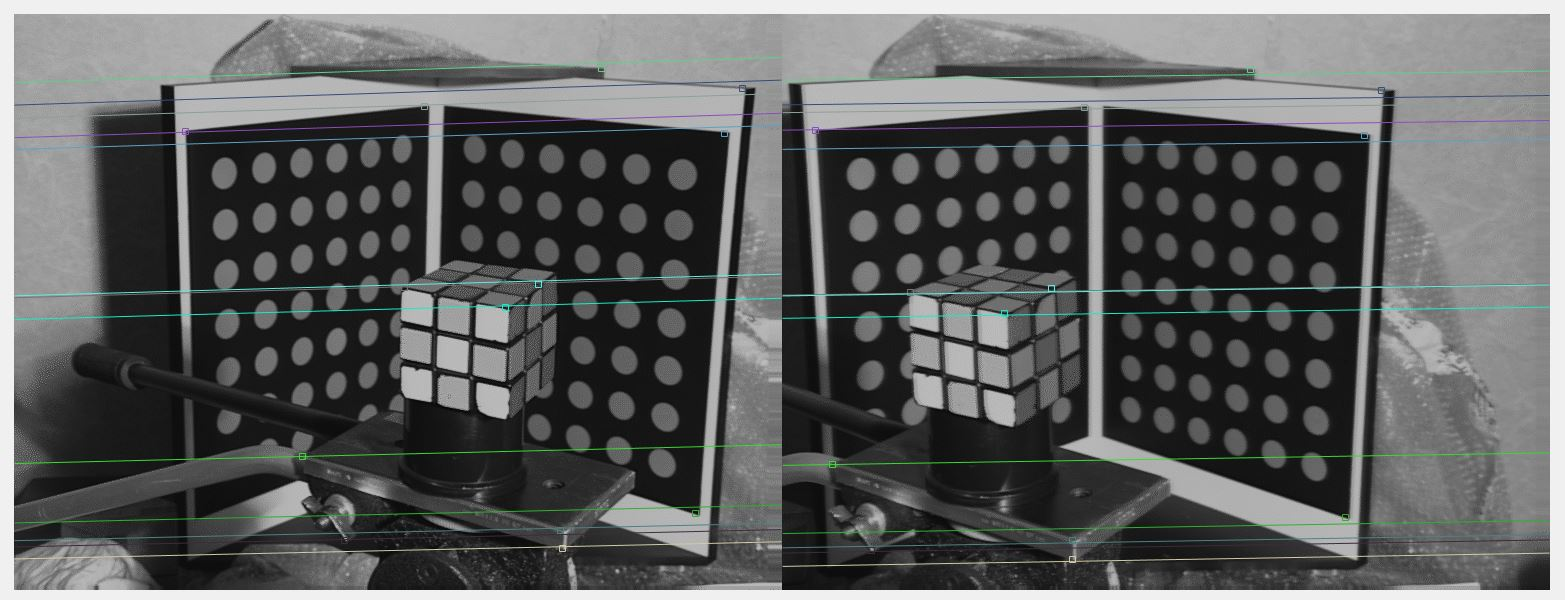
\includegraphics[width = \textwidth]{Resources/F1.jpg}
    \caption{Rubik epipolar lines for the algorithm version1}
    \label{fig:Rubik epipolar lines for the algorithm version1}
\end{figure}

\begin{figure} [ht]
    \centering
    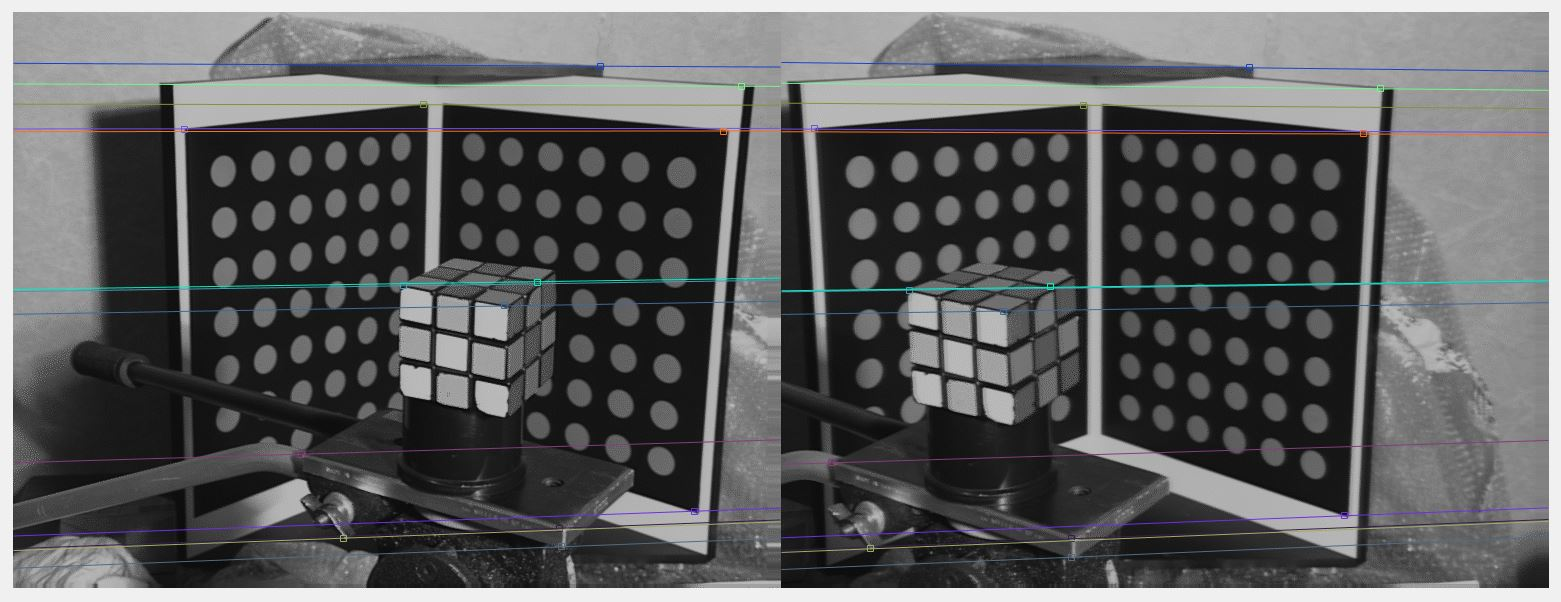
\includegraphics[width = \textwidth]{Resources/F2.jpg}
    \caption{Rubik epipolar lines for the algorithm version2}
    \label{fig:Rubik epipolar lines for the algorithm version2}
\end{figure}

As a consequence of this, the epipolar lines are depicted with a lower degree of precision in Figure 1, which does not have any normalized corresponding points, in comparison to Figure 2, which contains normalized corresponding points. In this case, the epipolar lines do not cross exactly the points that correspond to them, whereas in normalized ones, the lines pass close to or through the correspondences with a higher degree of accuracy.

All of the procedures described above are performed for another photo that is referred to as "Mire," and the results are displayed in a manner that is crystal clear. In Figure 3, the epipolar lines are depicted using algorithm version 1, and in Figure 4, the normalized matching points are depicted in their respective illustrations.

Taking a look at the constraint equation for this collection of photographs, it is clear that the fundamental matrix for this collection is a more accurate estimation than Rubik's pictures. This is because the result of the error is significantly closer to zero than it is with Rubik's pictures.

It is important to point out that the Main script encompasses the codes that are developed for this particular section. As a result of commenting on the relative names of the photographs and their points and uncommenting the names of other images, it is possible to evaluate the functionality of these two methods on a variety of images.

\begin{equation*}
    X^TFX = 
    \begin{bmatrix}
        0.0072 & 0.0018 & 0.0073 & 0.0100 & 0.0227 & 0.0253 & 0.0252 & 0.0547 & 0.0246 & 0.0401 \\
        0.0427 & 0.00079 & 0.0192 & 0.0115 & 0.0010 
    \end{bmatrix}
\end{equation*}
    
\begin{equation*}
    X^TFX_N = 
    \begin{bmatrix}
        0.0094 & 0.0004 & 5.858 \times 10^{-06} & 0.0050 & 0.0031 & 0.0097 & 0.0048 & 0.0072 & 0.0030 & 0.0010 \\
        0.0092 & 0.0043 & 0.0021 & 0.0099 & 0.069
    \end{bmatrix}
\end{equation*}

\begin{figure} [ht]
    \centering
    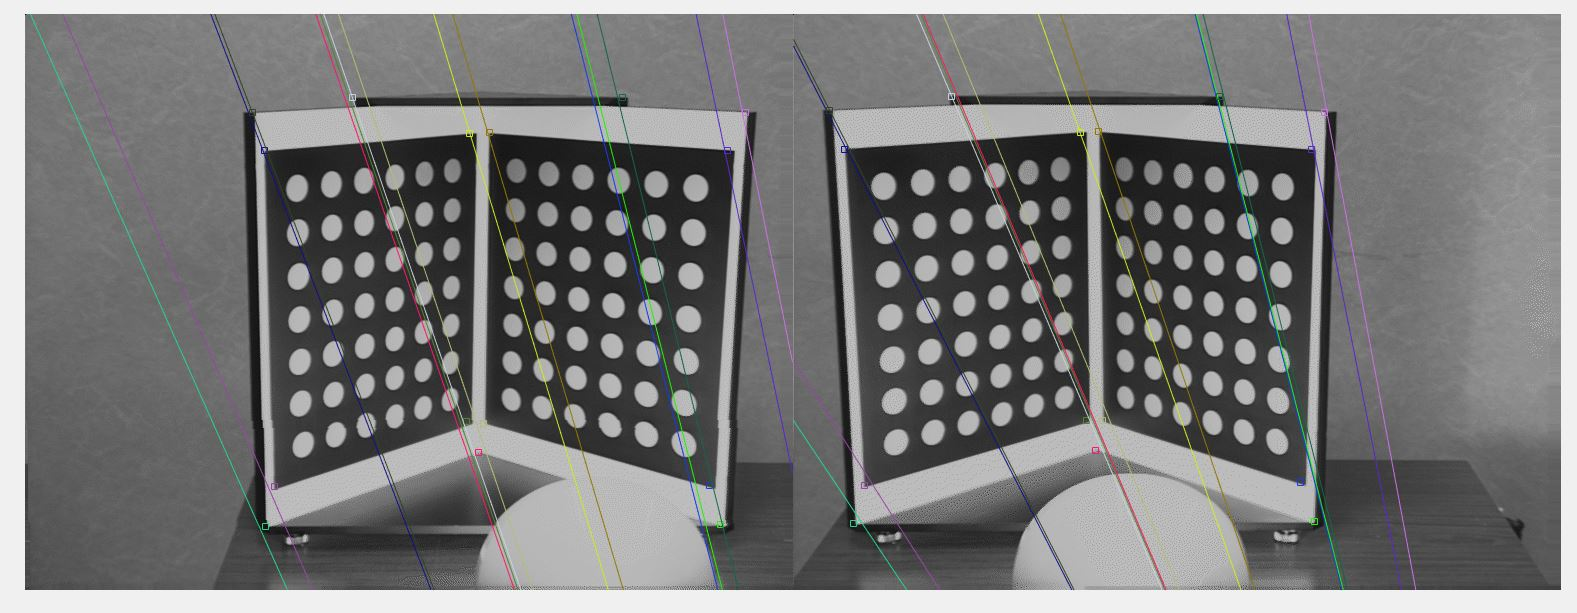
\includegraphics[width = \textwidth]{Resources/F3.jpg}
    \caption{Mire epipolar lines for the algorithm version1}
    \label{fig:Mire epipolar lines for the algorithm version1}
\end{figure}

\begin{figure} [ht]
    \centering
    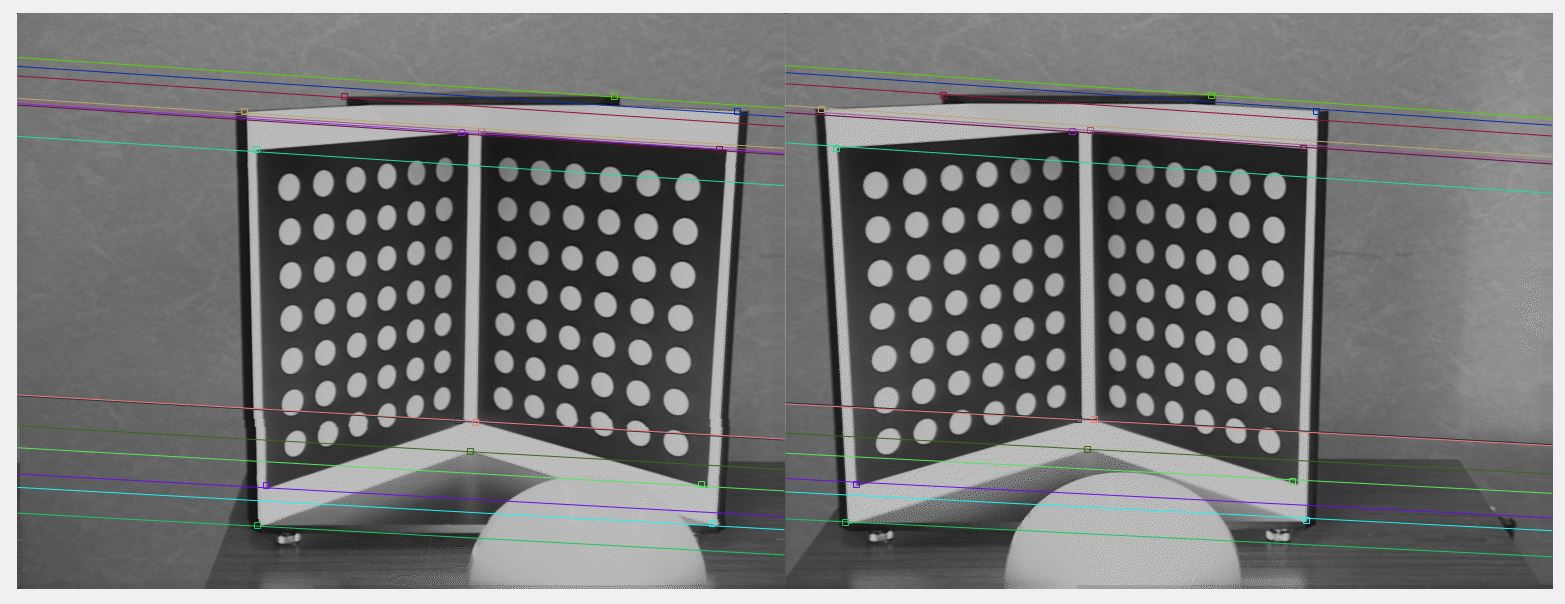
\includegraphics[width = \textwidth]{Resources/F4.jpg}
    \caption{Mire epipolar lines for the algorithm version2}
    \label{fig:Mire epipolar lines for the algorithm version2}
\end{figure}

Examining the epipoles reveals the same result as the previous procedure. Computing the left and right epipoles, which are the last columns of $U$ and $V$ in $\text{svd}(F)$, respectively, is the process that is carried out. It is also important that the left and right epipoles are aligned with the epipolar line. As a consequence of this, the epipolar constraint ought to be satisfied by these two epipoles ($e_l^T F e_r = 0$). After computing the value of this constraint for both fundamental matrices, it is found that both of them are extremely small. For example, the value for $F_1$ is $6.15 \times 10^{-22}$, and the value for $F_2$ is $9.8187 \times 10^{-25}$.